\documentclass{standalone}
\usepackage{tikz}
\usetikzlibrary{positioning,arrows.meta}
\begin{document}
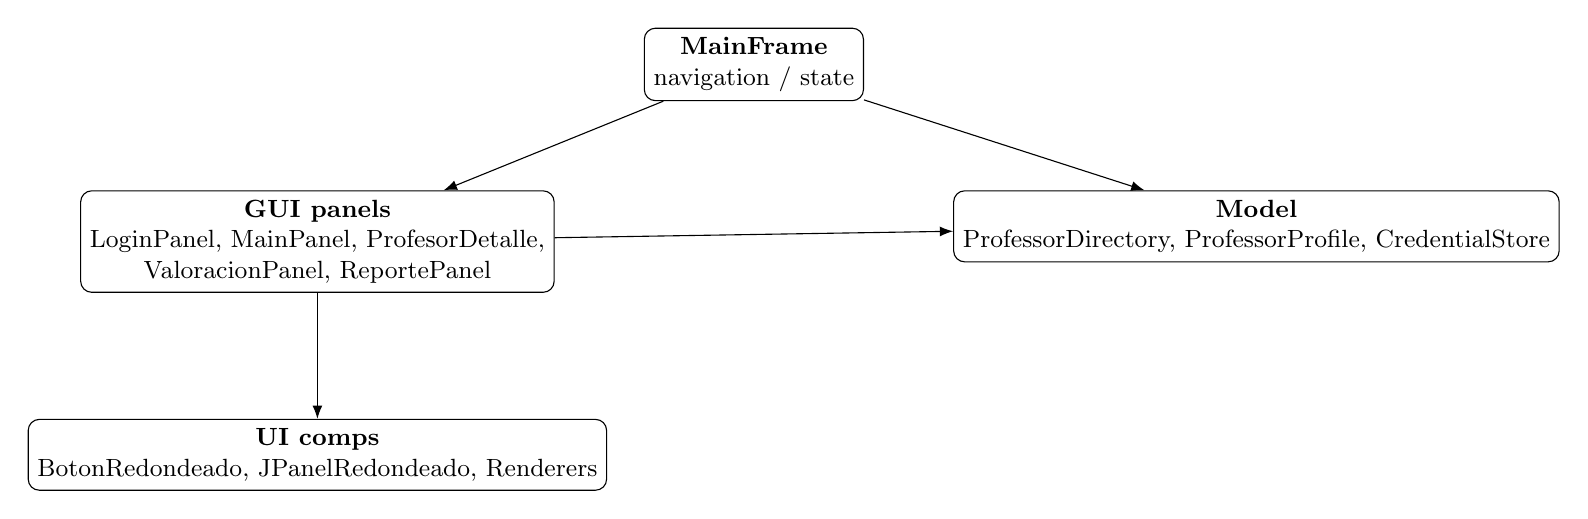
\begin{tikzpicture}[node distance=1.6cm, every node/.style={draw, rectangle, rounded corners, align=center, font=\small}]
    \node (MainFrame) {\textbf{MainFrame}\\navigation / state};
    \node (GUI) [below left=of MainFrame] {\textbf{GUI panels}\\LoginPanel, MainPanel, ProfesorDetalle,\\ValoracionPanel, ReportePanel};
    \node (Model) [below right=of MainFrame] {\textbf{Model}\\ProfessorDirectory, ProfessorProfile, CredentialStore};
    \node (UI) [below=of GUI] {\textbf{UI comps}\\BotonRedondeado, JPanelRedondeado, Renderers};

    \draw[->, -{Latex}] (MainFrame) -- (GUI);
    \draw[->, -{Latex}] (MainFrame) -- (Model);
    \draw[->, -{Latex}] (GUI) -- (UI);
    \draw[->, -{Latex}] (GUI) -- (Model);
\end{tikzpicture}
\end{document}
